\chapter{Ein allgemeiner Überblick über die germanischen Sprachen}

Dieses Kapitel gibt einen Überblick über allgemeine Fakten zu den germanischen\il{Germanisch} Sprachen. Es geht zurück auf
Folien für Lehrveranstaltungen über germanische\il{Germanisch} Sprachen, die von Ekkehard König verwendet und an
Matthias Hüning weitergegeben wurden und über Matthias an mich gelangten, was die Ähnlichkeit zum einführenden
Kapitel von \citet{HvDA94a} in dem von \citet{KvdA94a-ed} herausgegebenen Buch \emph{The Germanic Languages} erklärt.



\section{Sprachen und Sprecher*innen}

Je nachdem, wen man fragt, werden derzeit weltweit zwischen 5000 und 7000 Sprachen gesprochen. Die
germanischen\il{Germanisch} Sprachen bilden eine kleine Teilmenge davon, je nach Zählung 15--20 Sprachen, weil die Unterscheidung zwischen Sprache und Sprachvarietät nicht immer nach denselben Kriterien getroffen wird (\zb Varietäten des \ili{Niederländisch}en).
%AZ: (\zb varieties of \ili{Frisian}).AZ: I would not choose \ili{Frisian} as an example because some people might think of it as a variety of \ili{Dutch}.
Nach Max \citet[\page 13]{Weinreich45a-u} ist eine Sprache ein Dialekt mit einer Armee und einer
Marine. Nach dieser „Definition“ wäre weder das \ili{Jiddisch}e noch das \ili{Färöisch}e eine Sprache.\footnote{%
Siehe \citet[\page 13]{Weinreich45a-u} zum \ili{Jiddisch}en: \url{https://en.wikipedia.org/wiki/A_language_is_a_dialect_with_an_army_and_navy}.
}
%AZ The Swiss army has a bicycle group but the country has no navy.
%  https://de.wikipedia.org/wiki/Motorbootkompanie
%That the Swiss army has a bicycle group instead of a navy does not help.
%This brief discussion should indicate that
Es ist oft eine politische Frage, ob zwei eng verwandte Varianten einer Sprache als verschiedene Sprachen behandelt werden oder nicht (\ili{Slowakisch} vs.\ \ili{Tschechisch}, \ili{Serbisch} vs.\ \ili{Kroatisch}, \ili{Dänisch} vs.\ \ili{Norwegisch}).
Insgesamt haben die germanischen\il{Germanisch} Sprachen fast 500 Millionen Muttersprachler*innen, was 1/12 der gesamten Weltbevölkerung
entspricht. Besonders weit verbreitet ist das \ili{Englisch}e, das in sehr vielen Regionen
gesprochen wird.


\section{Historische Anmerkungen und Verwandtschaft zwischen den Sprachen}


Die germanischen\il{Germanisch} Sprachen bilden einen eigenen Zweig des Baums, der die indoeuropäische\il{Indoeuropäisch}
Sprachfamilie darstellt \citep[\page 665]{Fitch2007a-u}.
%(see Figure~\vref{fig-indo-european-fitch}).\footnote{
% The tree is a simplification ignoring many many languages. The sizes of the branches do not
% correspond to the number of speakers.
% \begin{figure}
% \includegraphics[width=\textwidth]{Pictures/indoeuropaeisch}
% \caption{\label{fig-indo-european-fitch}Language tree according to \citet[\page 665]{Fitch2007a-u}}
% \end{figure}
Das \ili{Urgermanisch}e bildete sich zwischen 2000 und
1000 v.\,Chr. heraus. Seine Ursprünge liegen im Ostseeraum, das heißt im nördlichen Deutschland und im südlichen
Skandinavien. Um 500 v.\,Chr. erstreckte sich das Gebiet, in dem es gesprochen wurde, von der Nordsee bis nach Polen.
Die ersten schriftlichen Zeugnisse sind Runen aus etwa 300 n.\,Chr. und die gotische\il{Gotisch} Bibelübersetzung im vierten Jahrhundert.
Die erste germanische\il{Germanisch} Lautverschiebung fand vor dem zweiten Jahrhundert v.\,Chr. statt. In diesem Jahrtausend entwickelten die
germanischen\il{Germanisch} Sprachen andere Konsonanten als die übrigen indoeuropäischen\il{Indoeuropäisch} Sprachen.

\citet[\page 8]{Harbert2006a-u} stellt die Abbildung~\vref{fig-history-relations-germanic} bereit, die die Entwicklung der
germanischen\il{Germanisch} Sprachen darstellt.
\begin{figure}
%\begin{sideways}
%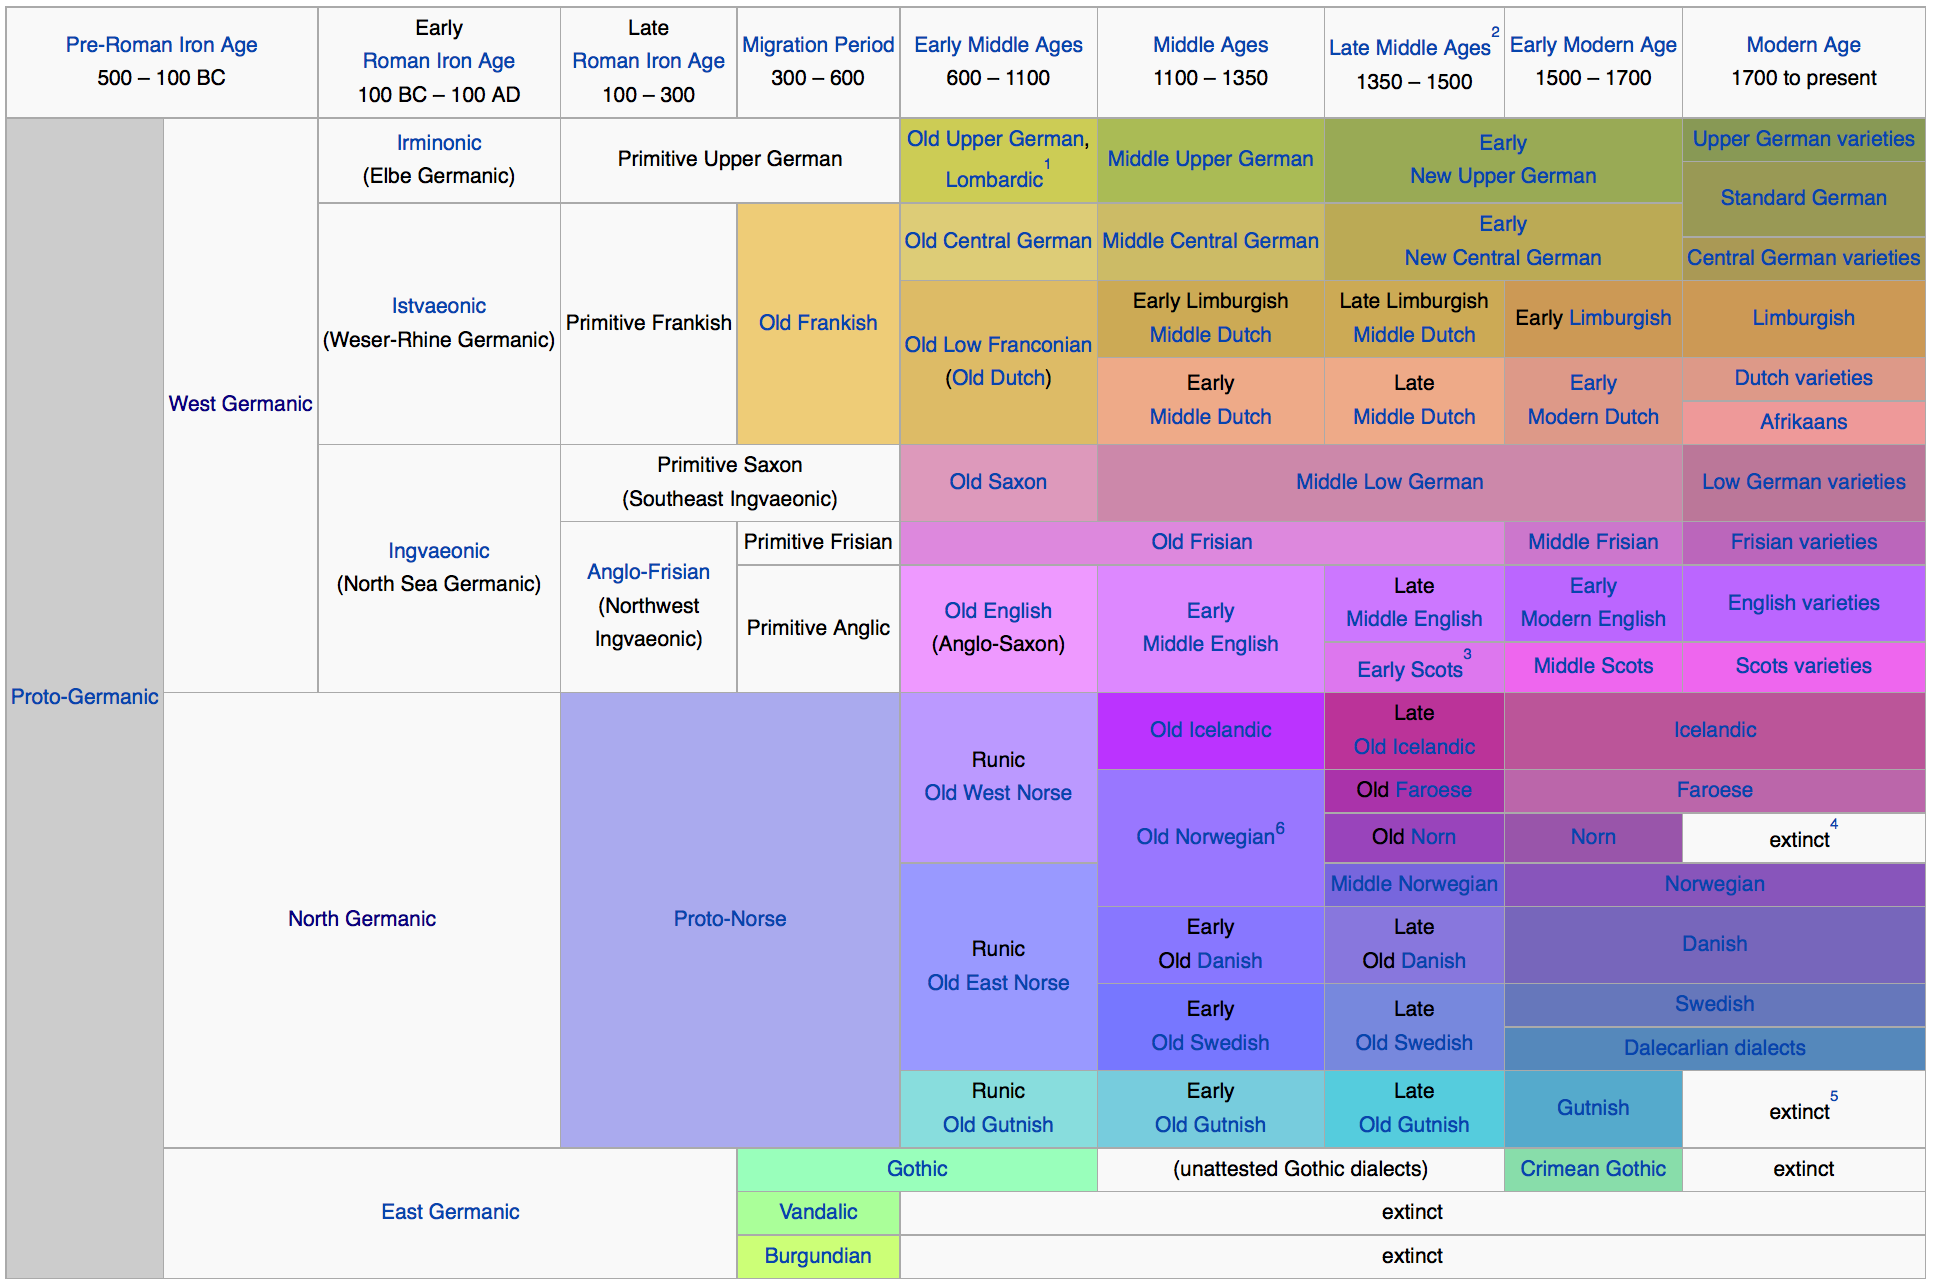
\includegraphics[width=.9\textheight]{Pictures/germanic-wikipedia}
%\end{sideways}
\begin{sideways}
\scalebox{.72}{%
% \begin{forest}forked edges, for tree={grow'=0, child anchor=west, parent anchor=east, align=center}
% [Proto-Germanic\il{Germanic!Proto-}
%     [Northwest Germanic\il{Germanic!Northwest}
%         [North Germanic\il{Germanic!North}, tier=preroman
%             [Old Norse\il{Norse!Old}
%                 [West Norse\il{Norse!West}, tier=premodern
%                     [\ili{Icelandic}, tier=modern]
%                     [\ili{Farocese}, tier=modern]
%                     [\ili{Norwegian}, tier=modern
%                         [\ili{Nynorsk}]
%                     ]
%                 ]
%                 [East Norse\il{Norse!East}
%                     [\ili{Danish}, tier=modern
%                         [\ili{Bokmål}]
%                     ]
%                     [\ili{Swedish}, tier=modern]
%                 ]
%              ]   
%         ]
%         [West Germanic\il{Germanic!West}, tier=preroman
%             [North Sea Germanic\il{Germanic!North Sea}\\(Ingvaeonic)
%                 [Anglo-Frisian\il{Frisian!Anglo-}
%                         [\ili{English}, tier=modern]
%                         [\ili{Frisian}, tier=modern]
%                 ]        
%                 [Old Saxon\il{Saxon!Old}
%                     [Low German\il{German!Low}, tier=modern]
%                 ]
%             ]
%             [\ili{Franconian}\\(Istvaeonic)
%                 [Low Franconian\il{Franconian!Low}, tier=middleages
%                     [Middle Dutch\il{Dutch!Middle}, tier=latemiddleages
%                         [\ili{Dutch}, tier=modern]
%                         [\ili{Afrikaans}, tier=modern]
%                     ]
%                 ]
%                 [High Franconian\il{Franconian!High}, tier=middleages, name=franconian
%                 ]
%             ]
%             [Alpine Germanic\il{Germanic!Alpine}\\(Irminonic)
%                 [\ili{Alemannic}\\\small{(Upper German\il{German!Upper})}, tier=middleages, name=alemannic
%                 	[Middle High\\German\il{German!Middle High}, tier=latemiddleages, no edge, name=mhg 
%                 		[High German\il{German!High}, tier=modern]
%                 		[PA German\il{Pennsylvania German}, tier=modern]
%                 		[\ili{Yiddish}, tier=modern]
%                 	]
%                 ]               
%                 [\ili{Bavarian}\\\small{(Upper German)\il{German!Upper}}, tier=middleages, name=bavarian]
%             ]
%         ]
%     ]    
%     [East Germanic\il{Germanic!East},  tier=preroman
%         [\ili{Gothic} (and others)]
%     ]
% ]
% {\draw[black] (franconian.east)--(mhg.west);}
% {\draw[black] (bavarian.east)--(mhg.west);}
% {\draw[black] (alemannic.east)--(mhg.west);}
% \end{forest}}
\begin{forest}forked edges, for tree={grow'=0, child anchor=west, parent anchor=east, align=center}
[Proto-Germanic
    [Northwest Germanic
        [North Germanic, tier=preroman
            [Old Norse
                [West Norse, tier=premodern
                    [Icelandic, tier=modern]
                    [Faroese, tier=modern]
                    [Norwegian, tier=modern
                        [Nynorsk]
                    ]
                ]
                [East Norse
                    [Danish, tier=modern
                        [Bokmål]
                    ]
                    [Swedish, tier=modern]
                ]
             ]   
        ]
        [West Germanic, tier=preroman
            [North Sea Germanic\\(Ingvaeonic)
                [Anglo-Frisian
                        [English, tier=modern]
                        [Frisian, tier=modern]
                ]        
                [Old Saxon
                    [Low German, tier=modern]
                ]
            ]
            [Franconian\\(Istvaeonic)
                [Low Franconian, tier=middleages
                    [Middle Dutch, tier=latemiddleages
                        [Dutch, tier=modern]
                        [Afrikaans, tier=modern]
                    ]
                ]
                [High Franconian, tier=middleages, name=franconian
                ]
            ]
            [Alpine Germanic\\(Irminonic)
                [Alemannic\\\small{(Upper German)}, tier=middleages, name=alemannic
                	[Middle High\\German, tier=latemiddleages, no edge, name=mhg 
                		[High German, tier=modern]
                		[PA German, tier=modern]
                		[Yiddish, tier=modern]
                	]
                ]               
                [Bavarian\\\small{(Upper German)}, tier=middleages, name=bavarian]
            ]
        ]
    ]    
    [East Germanic,  tier=preroman
        [Gothic (and others)]
    ]
]
{\draw[black] (franconian.east)--(mhg.west);}
{\draw[black] (bavarian.east)--(mhg.west);}
{\draw[black] (alemannic.east)--(mhg.west);}
\end{forest}}
\end{sideways}
% Index entries have to be outside the figure if/since memoize is used
\il{Deutsch!Mittelhoch-}\il{Deutsch!Ober-}\il{Deutsch!Mittelhoch-}\il{Deutsch!Ober-}\il{Bairisch}\il{Germanisch!Alpen-}\il{Afrikaans}%
\il{Alemannisch}\il{Germanisch!Ur-}\il{Germanisch!Nordwest-}\il{Germanisch!Nord-}\il{Nordisch!Alt-}\il{Nordisch!West-}\il{Isländisch}%
\il{Färöisch}\il{Norwegisch}\il{Nynorsk}\il{Nordisch!Ost-}\il{Dänisch}\il{Bokmål}\il{Schwedisch}\il{Germanisch!West-}\il{Germanisch!Nordsee-}%
\il{Friesisch!Angel-}\il{Englisch}\il{Friesisch}\il{Sächsisch!Alt-}\il{Deutsch!Nieder-}\il{Fränkisch}\il{Fränkisch!Nieder-}\il{Niederländisch!Mittel-}%
\il{Niederländisch}\il{Afrikaans}\il{Fränkisch!Hoch-}\il{Alemannisch}\il{Deutsch!Hoch-}\il{Pennsylvania-Deutsch}\il{Jiddisch}\il{Bairisch}%
\il{Germanisch!Ost-}\il{Gotisch}%
\caption{\label{fig-history-relations-germanic}Entwicklung der germanischen Sprachen nach
  \citew[\page 8]{Harbert2006a-u}}
\end{figure}
Das \ili{Germanisch}e wird in Ost\il{Germanisch!Ost}-, West\il{Germanisch!West}- und
Nord\il{Germanisch!Nord}germanisch eingeteilt. Das Ostgermanische existierte in Form des \ili{Gotisch}en
bis etwa 1800 auf der Krim (Krimgotisch\il{Gotisch!Krim-}) und ist heute vollständig ausgestorben.

Das Westgermanische\il{Germanisch} besteht aus
\begin{itemize}
\item \ili{Deutsch},
\item \ili{Jiddisch},
\item \ili{Luxemburgisch},
\item \ili{Pennsylvania-Dutch},
\item Niederdeutsch\il{Deutsch!Nieder-}, % Plattdeutsch or Niederdeutsch
\item \ili{Plautdietsch} (auch Mennonitisches Niederdeutsch\il{Deutsch!Mennonitisches Nieder-} genannt), %
\item \ili{Niederländisch},
\item \ili{Afrikaans},
\item \ili{Friesisch} und
\item \ili{Englisch}.
\end{itemize}
%\largerpage
Die nordgermanischen\il{Germanisch} Sprachen sind:
\begin{itemize}
\item \ili{Dänisch},
\item \ili{Schwedisch},
\item \ili{Norwegisch},
\item \ili{Isländisch} und
\item \ili{Färöisch}.
\end{itemize}

\noindent
Tabelle~\vref{tab-words-germanic} zeigt, wie ähnlich die Wörter aus dem Grundwortschatz der germanischen\il{Germanisch}
Sprachen sind:
\begin{table}
\centerfit{%
\begin{tabular}{lllllllll}
\hline\hline
\ili{Niederländisch} & vader  & vier    & vol    & huis  & bruin  & uit & kruid     & muis\\
\ili{Deutsch}        & Vater  & vier    & voll   & Haus  & braun  & aus & Kraut     & Maus\\
\ili{Englisch}       & father & four    & full   & house & brown  & out & crowd (?) & mouse\\
\ili{Friesisch}      & –      & fjouwer & fol    & hûs   & brún   & út  & krûd      & mûs\\
\ili{Schwedisch}     & fader  & fyra    & full   & hus   & brun   & ut  & krut      & mus\\
\ili{Dänisch}        & fader  & fire    & fuld   & hus   & brun   & ud  & krudt     & mus\\
\ili{Norwegisch}     & far    & fire    & full   & hus   & brun   & ut  & krydder   & mus\\
\ili{Isländisch}     & faðir  & fjórir  & fullur & hús   & brúnn  & út  & –         & mús\\
\hline\hline
\end{tabular}
}
\caption{\label{tab-words-germanic}Wörter aus dem Grundwortschatz einiger germanischer Sprachen}
\end{table}

%% \section{Stammbaum der germanischen Sprachen}
%% \includegraphics[width=\textwidth]{Pictures/stammbaum-germanisch}
%% aus \citew[S.\,251]{Bussmann2002a}





\section{Die drei Zweige der germanischen Familie}

Das \ili{Urgermanisch}e entwickelte sich etwa im ersten Jahrhundert n.\,Chr. zu den drei Hauptzweigen Ost-, West- und Nordgermanisch\il{Germanisch}. Die Gründe für diese Entwicklung waren inhärente Variationen in den jeweiligen
Dialekten, Migration (Sprachkontakt) und Standardisierung. Das vorliegende Buch behandelt die Struktur der
germanischen\il{Germanisch} Standardsprachen. Dieser Abschnitt ist in drei Unterabschnitte gegliedert, die den
drei germanischen Hauptzweigen entsprechen. Ich werde die historischen Entwicklungen skizzieren, die zu den
heute gesprochenen Sprachen geführt haben. Viele der Details, die in Abbildung~\ref{fig-history-relations-germanic} dargestellt sind, werden dabei ignoriert.



\subsection{Ostgermanisch}

Es\il{Germanisch!Ost|(} wird oft behauptet, dass die Goten von den dänischen\il{Dänisch} Inseln und aus Südschweden auf das europäische Festland
auswanderten, doch neuere Forschung, die archäologische Funde berücksichtigt, geht davon aus, dass sie
im ersten Jahrhundert n.\,Chr. auf dem europäischen Festland gegenüber Skandinavien rund um die Weichsel lebten und später nach Süden in das Hinterland des
Schwarzen Meeres zogen \citep[20--30]{Heather1999a-u}. In dieser Zeit standen sie in Kontakt mit den Vandalen\il{Vandalisch} und anderen Stämmen.
%emigrated from the \ili{Danish} islands and South Sweden around 100 BCE and met the
%Vandals and other tribes.\itdopt{%
%Walkden: Most current historical research (since e.g. Heather 1998, The Goths, 25–30) rejects the
%idea that the Goths originated in Scandinavia, and put their earliest origin around the Vistula. Not
%a crucial point in the context of this book, but may be worth changing.
%}
Das \ili{Gotisch}e, \ili{Vandalisch}e und \ili{Burgundisch}e sowie einige kleinere Sprachen bildeten den ostgermanischen Zweig, von dem nur das \ili{Gotisch}e überliefert wurde.
Nach dem Zerfall der gotischen\il{Gotisch} Reiche starb das \ili{Gotisch}e aus. Auf der Halbinsel Krim gab es einige Überreste
bis etwa 1800. Der westgotische\il{Gotisch} Bischof Wulfila (oder vielmehr ein von ihm geleitetes Team, siehe
\citealt{Ratkus2018a-u}) übersetzte die Bibel ins \ili{Gotisch}e. Die
bekannteste Fassung davon ist das Fragment Codex Argenteus, das sich in der Universitätsbibliothek von
Uppsala befindet. Abbildung~\vref{fig-Wulfila-Bibel} zeigt ein Bild davon.\footnote{
Übernommen aus Wikipedia: \url{http://de.wikipedia.org/wiki/Bild:Wulfila_bibel.jpg}. 19.10.2014.
}
\begin{figure}
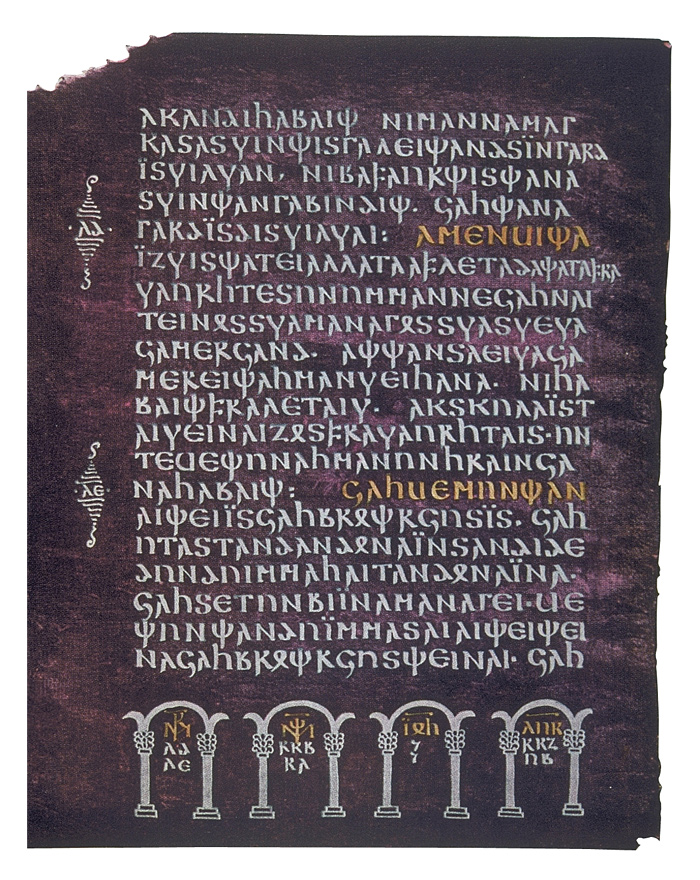
\includegraphics[width=53mm]{Pictures/Wulfila_bibel}
\caption{\label{fig-Wulfila-Bibel}Die Wulfila-Bibel (Codex Argenteus), Bild aus Wikipedia}
\end{figure}
\il{Germanisch!Ost|)}


\subsection{Nordgermanisch}

Die\il{Germanisch!Nord|(} ersten Schriften auf Runensteinen gehen auf das sechste Jahrhundert zurück. Die Sprache der Wikinger
(800--1050) war recht homogen, und erst nach dieser Epoche begannen sich zwei Zweige zu
entwickeln: der ostskandinavische\il{Skandinavisch!Ost} Zweig mit Altdänisch\il{Dänisch!Alt-} und Altschwedisch\il{Schwedisch!Alt-} und der westskandinavische\il{Skandinavisch!West} Zweig
mit Altnorwegisch\il{Norwegisch!Alt-} und Altisländisch\il{Isländisch!Alt-}.


\subsubsection{Dänisch}

Das \ili{Dänisch}e (dansk) ist die Amtssprache des
\href{https://en.wikipedia.org/wiki/Denmark}{Königreichs Dänemark} und die zweite Amtssprache der
Färöer-Inseln und Grönlands, wobei das \ili{Grönländisch}e die erste Amtssprache
Grönlands ist. Das \ili{Dänisch}e hat etwa 5,5 Millionen Sprecher*innen. Etwa 50.000 Sprecher*innen leben in \href{https://en.wikipedia.org/wiki/Schleswig-Holstein}{Schleswig-Holstein}, dem nördlichsten der Bundesländer Deutschlands.
Das \ili{Dänisch}e ist die skandinavische\il{Skandinavisch} Sprache, die sich am weitesten von den gemeinsamen skandinavischen\il{Skandinavisch} Wurzeln entfernt hat.


\subsubsection{Schwedisch}

Das \ili{Schwedisch}e (svenska) ist die Amtssprache in Schweden mit etwa 8,5 Millionen Muttersprachler*innen. Es ist
die Erstsprache von etwa 300.000 schwedischsprachigen\il{Schwedisch} Finnen in Finnland. Bis in die Zeit der
Wikinger waren das \ili{Dänisch}e und das \ili{Schwedisch}e kaum zu unterscheiden. Ab etwa 800 begannen sie
auseinanderzudriften. Seit etwa 1300 gibt es deutliche Unterschiede.



\subsubsection{Isländisch}


Das \ili{Isländisch}e (íslenska) wird seit der Besiedlung Islands vor über 1000 Jahren dort
gesprochen. Mit dem \ili{Färöisch}en gehört es zu den westskandinavischen Sprachen\il{Skandinavisch!West-}.
% Wikipedia 23.10.2014
Es gibt etwa 325.000 Muttersprachler*innen. 97\,\% der isländischen\il{Isländisch} Bevölkerung (325.000) haben das \ili{Isländisch}e als
Muttersprache, und es gibt große Gruppen von Muttersprachler*innen in Dänemark, den USA und Kanada
(insgesamt etwa 15.000).
Es gibt weniger Variation als in anderen germanischen\il{Germanisch} Sprachen (keine Dialekte).
%AZ that is too strong there is actually quite a bit of variation but maybe it is correct to say that there is less variation than in other \ili{Germanic} languages
Die Sprache ist konservativ in dem Sinne, dass das \ili{Isländisch}e
diejenige unter den germanischen\il{Germanisch} Sprachen ist, die den germanischen\il{Germanisch} Wortschatz und die Flexion am besten bewahrt hat.
Am Anfang gab es kaum Unterschiede zwischen dem \ili{Norwegisch}en und dem \ili{Isländisch}en, aber
% The \ili{Dano-Norwegian}, then later \ili{Danish} rule of Iceland from 1536 to 1918 had little effect on the
% evolution of \ili{Icelandic} (in contrast to the \ili{Norwegian} language), which remained in daily use among
% the general population.
% AZ: when?
ab etwa 1100 drifteten die Sprachen auseinander. Dieser Prozess setzte sich auch aufgrund des dänischen\il{Dänisch}
Einflusses fort, und heutzutage ähnelt das \ili{Norwegisch}e mehr dem \ili{Dänisch}en als dem
\ili{Isländisch}en. Es gibt viele isländische\il{Isländisch} Schriftzeugnisse.

\subsubsection{Norwegisch}

%\largerpage
Es gibt zwei Standardvarietäten des \ili{Norwegisch}en (norsk): Dänisch-Norwegisch\il{Norwegisch!Dänisch-} (bokmål) und Neunorwegisch\il{Norwegisch!Neu-} (nynorsk, landsmål).
Beide sind Amtssprachen Norwegens.
% and are used in parallel\itdopt{AZ: not clear what that means}.
Es gibt etwa 4,3 Millionen Sprecher*innen.
Von 1380 bis 1814 war das \ili{Dänisch}e die Schriftsprache, und in Norwegen wurden lokale Dialekte gesprochen. Daraus entwickelte sich der Bokmål-Standard.
Ivar Aasen (1813--1896) entwickelte mit \ili{Nynorsk} einen Standard, der weniger vom \ili{Dänisch}en beeinflusst ist. \ili{Nynorsk} erhielt 1885 offiziellen Status. Das \ili{Bokmål} `Buchsprache' ist die Erstsprache der meisten
Norweger.

\subsubsection{Färöisch}

Das \ili{Färöisch}e (føroyskt) ist -- neben dem \ili{Dänisch}en -- Amtssprache der Färöer-Inseln. Es
gibt etwa 47.000 Sprecher*innen. Die Färöer-Inseln gehören seit 1816 zu Dänemark. Seit 1948 sind sie
ein selbstverwaltetes Land innerhalb des \href{https://en.wikipedia.org/wiki/Danish_Realm}{dänischen\il{Dänisch} Reichs}.
Das \ili{Färöisch}e hat einen starken dänischen\il{Dänisch} Einfluss. Die erste handschriftliche Überlieferung stammt erst aus dem Jahr 1773, und
auch nach diesem Datum gibt es nicht viele schriftliche Zeugnisse.%
%AZ i would leave this out: (in contrast to \ili{Icelandic}).And put something in the \ili{Icelandic} section
\il{Germanisch!Ost|)}

\subsection{Westgermanisch}


Die\il{Germanisch!West|(} Meinungen zu der Frage, ob sich das Westgermanische aus einer einzigen Quelle entwickelt hat oder nicht, gehen auseinander. Einige Autoren
nehmen an, dass die westgermanischen\il{Germanisch} Sprachen keine gemeinsame Wurzel haben, sondern sich aus den
folgenden drei nicht verwandten Zweigen von Dialektgruppen entwickelt haben (zum Beispiel \citealp[\page 17--18]{Robinson1992a-u} und
\citealp[\page 9]{HvDA94a}):
\begin{itemize}
\item Nordseegermanisch\il{Germanisch!Nordsee} %(Ingvaeonic, ancestral to \ili{Anglo-Frisian} and also Old Saxon)
\item Weser-Rhein-Germanisch\il{Germanisch!Weser-Rhein} %(Istvaeonic, ancestral to Old \ili{Frankish},
                                %its successors \ili{Low Franconian} and several dialects of Old High \ili{German})
\item Elbgermanisch\il{Germanisch!Elb-} %(Irminonic, ancestral to several dialects of Old High \ili{German}, most probably including the extinct \ili{Langobardic} language).
\end{itemize}
Andere Autoren nehmen an, dass diese drei Zweige einen gemeinsamen Vorfahren hatten (siehe
Abbildung~\ref{fig-history-relations-germanic}), und manche lehnen es ab, das Westgermanische überhaupt in
drei Unterzweige zu unterteilen \citep{Stiles2013a-u}.
Es gibt keine eindeutige Zuordnung dieser Dialektgruppen zu den heute gesprochenen Sprachen.%

%\largerpage
\subsubsection{Deutsch}

Das \ili{Deutsch}e ist die Amtssprache von
\begin{itemize}
\item Deutschland (etwa 80 Millionen Sprecher*innen),
\item Österreich (etwa 7,5 Millionen Sprecher*innen),
\item Liechtenstein (etwa 15.000 Sprecher*innen),
\item der Schweiz (4,2 Millionen von 6,4 Millionen Einwohnern der Schweiz),
\item Norditalien/Südtirol (etwa 270.000 Sprecher*innen),
\item Belgien (etwa 65.000 Sprecher*innen) und
\item Luxemburg (etwa 360.000 Sprecher*innen).
\end{itemize}
Neben dem \ili{Deutsch}en hat Luxemburg auch das \ili{Luxemburgisch}e und das \ili{Französisch}e als
Amtssprachen.
%Poland 50,000 native speakers.
Es gibt weitere Länder, in denen das \ili{Deutsch}e eine Nationalsprache oder eine nationale oder regionale
Minderheitensprache ist: Brasilien, Tschechien, Dänemark, Ungarn, Namibia, Polen, \ili{Rumänien}, Russland und die Slowakei.

% There are about 97 million speakers of \ili{German}, about, 90 of those are native speakers and 7 million
% have \ili{German} as their second language.
% % = Migrationshintergrund
% % Quelle Wikipedia 15.10.2013
% Approximately 80 million speakers speak \ili{German} as a foreign language, about 55 Million of these live
% in the \ili{European} Union.%AZ It is a bit awkward to get these details for \ili{German} but not for all the other languages

Es gibt drei nationale Hauptvarianten (Deutschland, Österreich, Schweiz). In anderen Ländern ist das \ili{Deutsch}e
%AZ leave out usually
eine Minderheitensprache. Es gibt zwei große Dialektgruppen: das Niederdeutsche\il{Deutsch!Nieder-}
(Plattdütsch, Plattdütsk, Plattduitsch, 
Nedderdütsch; im Standarddeutschen: Platt\-deutsch oder Nie\-der\-deutsch%
%AZ this is clear as mud: do you
%want to say that \ili{Dutch} is part of low Saxon or as most people do
%that low saxon are the dialects of \ili{German} that are spoken in in the Netherlands? I would say:
%Nedersaksisch or Low Saxon, a group of dialects spoken in the Netherlands, southern Danmark and
%northwestern Germany
% Well, the areas in which Low Saxon is spoken overlap with national border. I speak about langauges
% spoken in these national borders here.
) und das Hochdeutsche\il{Deutsch!Hoch-} (Varietäten des \ili{Deutsch}en, die südlich der Benrather und Uerdinger
Isoglossen gesprochen werden).
%\itdopt{Stefan: fix}
%\todostefan{more}

% Wikipedia
%% The High \ili{German} languages or High \ili{German} dialects (\ili{German}: Hochdeutsche Dialekte) comprise the varieties of \ili{German} spoken south of the Benrath and Uerdingen isoglosses in central and southern Germany, Austria, Liechtenstein, Switzerland, and Luxembourg as well as in neighboring portions of Belgium (Eupen-Malmedy) and the Netherlands (Southeast Limburg), France (Alsace and northern Lorraine), Italy (South Tyrol), and Poland (Upper Silesia). They are also spoken in diaspora in \ili{Romania}, Russia, the United States, Brazil, Argentina, Chile, and Namibia.

%% The High \ili{German} languages are marked by the High \ili{German} consonant shift, separating them from Low \ili{German} and Low \ili{Franconian} (\ili{Dutch}) within the continental West \ili{Germanic} dialect continuum.


%% Wikipedia

%% \ili{Middle} Low \ili{German} was the lingua franca of the Hanseatic League. It was the predominant language in \ili{Northern} Germany. This changed in the 16th century: in 1534 the Luther Bible was published. This translation is considered to be an important step towards the evolution of the Early New High \ili{German}. It aimed to be understandable to a broad audience and was based mainly on Central and Upper \ili{German} varieties. The Early New High \ili{German} language gained more prestige than Low \ili{German} and became the language of science and literature. Around the same time, the Hanseatic league, based around northern ports, lost its importance as new trade routes to Asia and the Americas were established, while the most powerful \ili{German} states of that period were located in \ili{Middle} and Southern Germany.

%% The 18th and 19th centuries were marked by mass education in Standard \ili{German} in schools. Gradually Low \ili{German} came to be politically viewed as a mere dialect spoken by the uneducated. Today Low Saxon can be divided in two groups: Low Saxon varieties with a reasonable standard \ili{German} influx[clarification needed] and varieties of Standard \ili{German} with a Low Saxon influence known as Missingsch. Sometimes, Low Saxon and Low \ili{Franconian} varieties are grouped together because both are unaffected by the High \ili{German} consonant shift. However, the proportion of the population who can understand and speak it has decreased continuously since World War II.


%% Wikipedia
%% High \ili{German} is divided into Central \ili{German}, High \ili{Franconian} (a transitional dialect), and Upper \ili{German}. Central \ili{German} dialects include \ili{Ripuarian}, Moselle \ili{Franconian}, Rhine \ili{Franconian}, Central Hessian, East Hessian, North Hessian, Thuringian, \ili{Silesian} \ili{German}, Lorraine \ili{Franconian}, \ili{Mittelalemannisch}, North Upper Saxon, High \ili{Prussian}, Lausitzisch-Neumärkisch and Upper Saxon. It is spoken in the southeastern Netherlands, eastern Belgium, Luxembourg, parts of France, and parts of Germany roughly between the River Main and the southern edge of the Lowlands. Modern Standard \ili{German} is mostly based on Central \ili{German}, although the common (but not linguistically correct) \ili{German} term for modern Standard \ili{German} is Hochdeutsch, that is, High \ili{German}.

%% The Moselle \ili{Franconian} varieties spoken in Luxembourg have been officially standardised and institutionalised and are usually considered a separate language known as \ili{Luxembourgish}.

%% The two High \ili{Franconian} dialects are East \ili{Franconian} and South \ili{Franconian}.

%% Upper \ili{German} dialects include \ili{Northern} Austro-Bavarian, Central Austro-Bavarian, Southern Austro-Bavarian, Swabian, East \ili{Franconian}, High \ili{Alemannic} \ili{German}, Highest \ili{Alemannic} \ili{German}, Alsatian and Low \ili{Alemannic} \ili{German}. They are spoken in parts of the Alsace, southern Germany, Liechtenstein, Austria, and the \ili{German}-speaking parts of Switzerland and Italy.

%% Wymysorys is a High \ili{German} dialect of Poland native to Wilamowice, and Sathmarisch and Siebenbürgisch are High \ili{German} dialects of \ili{Romania}. The High \ili{German} varieties spoken by Ashkenazi Jews (mostly in the former \ili{Russian} Empire) have several unique features, and are usually considered as a separate language, \ili{Yiddish}. It is the only \ili{Germanic} language that does not use the \ili{Latin} script as the basis of its standard alphabet.


\subsubsection{Jiddisch}

Das \ili{Jiddisch}e ist eine von vielen Sprachen, die in der jüdischen Diaspora gesprochen werden. Was die Sprecher*innenzahl betrifft,
gibt es keine verlässlichen Zahlen: Einige Quellen gehen davon aus, dass
1,5 Millionen Menschen diese Sprache aktiv oder passiv sprechen, wobei nur 500.000 Sprecher*innen die Sprache
aktiv im Alltag verwenden. Andere Quellen gehen von 4 Millionen
Sprecher*innen aus. In jedem Fall war die Zahl der \ili{Jiddisch}sprecher*innen vor 100 Jahren deutlich
höher: \citet[\page 6]{Birnbaum1915a-u} schätzte die Zahl der Sprecher*innen auf bis zu 12 Millionen. Die meisten von
ihnen lebten im Gebiet der Sowjetunion (über 7 Millionen), und es gab größere Gemeinschaften in den Vereinigten Staaten (über 2 Millionen), in Österreich-Ungarn
(1,5 bis 2 Millionen), \ili{Rumänien} (über 250.000), Großbritannien
(250.000), Palästina, Argentinien und Kanada (jeweils etwa 100.000). Siehe auch \citew{Schaefer2023a} für
Schätzungen der Sprecher*innenzahlen und weitere Literaturhinweise.

%7 million speakers of \ili{Yiddish} lived in Europe, most of them in the area of the Sovjet Union and in
%Austria-Hungary. At most 75,000 \ili{Yiddish} speakers are left in Western Europe.
Das \ili{Jiddisch}e hat seine Wurzeln
im mittelalterlichen \ili{Deutsch} mit Einflüssen aus dem \ili{Hebräisch}en und \ili{Aramäisch}en. Es ist außerdem von
romanischen Sprachen beeinflusst, insbesondere von altfranzösischen\il{Französisch!Alt-} und italienischen\il{Italienisch} Varietäten.


\subsubsection{Pennsylvania-Deutsch}

\ili{Pennsylvania-Deutsch} (\ili{Pensilfaanish}, Pensilfaanish Deitsch), das auch als \emph{Pennsylvania Dutch} bekannt ist, hat etwa 300.000
Muttersprachler*innen, die hauptsächlich in den USA leben. Die wichtigsten Regionen sind Pennsylvania, Ohio und
Indiana. Das Pennsylvania-Deutsche hat sich aus pfälzischen Dialekten entwickelt, die von
Einwanderern gesprochen wurden, die im 17.\ und 18.\ Jahrhundert nach Nordamerika kamen.
% Die ersten um 1683
Angehörige verschiedener protestantischer Religionsgemeinschaften (Mennoniten, Pietisten und so weiter) verließen Europa aus religiösen Gründen,
doch später folgten Einwanderer, die aus wirtschaftlichen Gründen kamen. Die Sprache wird heutzutage
hauptsächlich von Amischen und Mennoniten gesprochen. 




\subsubsection{Niederländisch}

Das \ili{Niederländisch}e (Nederlands) ist die Amtssprache der Niederlande und hat in diesem Land etwa 15 Millionen Sprecher*innen. \ili{Niederländisch} ist außerdem eine der Amtssprachen Belgiens mit etwa 6 Millionen Sprecher*innen.
%AZleave out: ; almost 4 million Walloones).
Es ist die alleinige Amts- und Unterrichtssprache in Surinam
%AZ leave out: which is independent since 1975,
% 60% of the population speak it as their mother tongue % wikipedia
% 24% speak it as a second language
sowie in \href{https://en.wikipedia.org/wiki/Aruba}{Aruba} und den \href{https://en.wikipedia.org/wiki/Netherlands_Antilles}{Niederländischen Antillen}.

%In Aruba, Curaçao and Sint Maarten, all parts of the Kingdom of the Netherlands, \ili{Dutch} is the official language but spoken as a first language by only 7% to 8% of the population,[56] although most native-born people on the islands can speak the language since the education system is in \ili{Dutch} at some or all levels.[57] The lingua franca of Aruba, Bonaire and Curaçao is Papiamento, a creole language that originally developed among the slave population. The population of the three northern Antilles, Sint Maarten, Saba, and Sint Eustatius, is predominantly \ili{English}-speaking.[44]

\subsubsection{Afrikaans}

Das \ili{Afrikaans} ist seit 1925 eine der Amtssprachen Südafrikas, das elf Amtssprachen hat.
Es gibt etwa 6,4 Millionen Muttersprachler*innen in Südafrika, was etwa 15\,\% der Bevölkerung entspricht,
und 150.000 in Namibia. Das \ili{Afrikaans} hat sich seit dem 17. Jahrhundert aus niederländischen\il{Niederländisch} Dialekten entwickelt und wird
seit irgendwann zwischen 1775 und 1850 als eigenständige Sprache angesehen
%\parencites[\page 99]{denBesten2012b-u}
\citep[\page 272]{denBesten2012a-u}.
% Oft wird gesagt, dass ab ca. 1775 von '\ili{Afrikaans}' gesprochen werden kann (Den Besten spricht aber noch vom 'Proto-Afrikaans'). Die Übergänge vom Kap-Niederländischen zum \ili{Afrikaans} sind natürlich fließend, aber um die Zeit herum, gibt es doch schon genügend dokumentierte Unterschiede, um zu sagen, dass \ili{Afrikaans} eine eigenständige Sprache geworden ist. Allerspätestens ab Mitte des 19. Jahhunderts ist dann aber auf jeden Fall eine eigene Sprache anzusetzen; da sind sich alle einig. Und 1925 wird das dann ja auch offizielle Amtssprache. 
Die verschiedenen in der Region gesprochenen afrikanischen Sprachen standen in Wechselwirkung mit dem \ili{Afrikaans}.
%AZ leave out: and its origins and resulted in a structural simplification in comparison to \ili{Dutch}
Heute hat das \ili{Englisch}e einen starken Einfluss.



\subsubsection{Friesisch}

Die drei Varietäten des \ili{Friesisch}en sind untereinander nicht verständlich. Es gibt das Nordfriesische\il{Friesisch!Nord-}, das von
etwa 10.000 Sprecher*innen hauptsächlich auf den nordfriesischen\il{Friesisch} Inseln Amrum, Sylt und Helgoland gesprochen wird. Das Ostfriesische\il{Friesisch!Ost-}
ist mit Ausnahme des \ili{Saterfriesisch}en ausgestorben, das in den drei Dörfern des Saterlandes
(Landkreis Cloppenburg) von zwischen 1.000 und 2.500 Menschen gesprochen wird.
% https://www.taz.de/!5834717 Inseln
Das Westfriesische\il{Friesisch!West-} wird in der nördlichen niederländischen\il{Niederländisch} Provinz Fryslân (Friesland) gesprochen und hat etwa 350.000
Muttersprachler*innen.



\subsubsection{Englisch}

Weltweit hatte das \ili{Englisch}e Ende des 20. Jahrhunderts etwa 570 Millionen Sprecher*innen
(337 Millionen Muttersprachler*innen, 235 Millionen Sprecher*innen mit \ili{Englisch} als \isi{Zweitsprache}\footnote{%
  Der Terminus \emph{Zweitsprache} bezeichnet eine Sprache, die Sprecher*innen im
  Alltag verwenden, weil diese Sprache in der Umgebung, in der sie leben, gesprochen wird. Ein Beispiel wären Sprecher*innen mit
  Türkisch als Erstsprache, die in Deutschland leben. Die deutsche Tradition unterscheidet
  \emph{Zweitsprache} von \emph{Fremdsprache}.%
}). Die Länder mit den meisten Muttersprachler*innen sind im Folgenden aufgeführt:
\begin{itemize}
\item USA: 227 Millionen,
\item Großbritannien: 57 Millionen,
\item Nigeria: 43 Millionen,
\item Kanada: 24 Millionen,
\item Australien: 17 Millionen,
\item Irland: 3,5 Millionen,
\item Neuseeland: 3,2 Millionen.
\end{itemize}
Es gibt viele nationale Varianten, die sich hauptsächlich in der Aussprache unterscheiden.
Zwischen 1 und 1,5 Milliarden Menschen verfügen über aktive oder passive Kenntnisse des \ili{Englisch}en.
Das \ili{Englisch}e ist in 59 Staaten Amtssprache. Es ist die wichtigste Wissenschaftssprache.%
\il{Germanisch!West|)}


\questions{
\begin{enumerate}
\item Nennen Sie mindestens zehn germanische Sprachen.
\end{enumerate}

}


%      <!-- Local IspellDict: de_DE -->
